\section{The ESP Cache Hierarchy}
\label{sec:cache}

The ESP cache hierarchy consists of L1/L2 caches and a LLC in order to achieve cache coherence on SoCs with multiple processors and accelerators. Figure ~\ref{fig:esp_hier} provides a high level functional view of each component of the hierarchy.
The directory controller refers to the LLC. The LLC interfaces directly with main memory, and services requests from private cache controllers or DMA controllers. 
The private cache controllers refer to the L1/L2 caches processors ($\mu$P) or accelerators, 
which service memory requests from the processors and sends requests to the LLC if needed. The DMA controller belongs to accelerators
without private caches. Rather than interfacing directly to main memory, these accelerators can receive data directly from the LLC if available.
\par Compared to the L1/L2 caches, the LLC contains additional metadata for the cache lines stored inside the L1/L2 caches at any point in time, such as which L1/L2 caches share the cache line or which L1/L2 owns the cache line. 
These metadata are necessary for the execution of the extended MESI directory-based cache coherence protocol. MESI stands for the four states that a cache line can be in at any point in time (Modified, Exclusive, Shared, Invalid).
The ESP LLC also maintains cache lines that are no longer being used by any L1/L2 cache in a Valid state. These cache lines are the first choice for evictions but can also be sent directly to accelerators if requested through DMA, which is 
much faster compared to accelerators reading the data directly from main memory. Valid cache lines can also be sent directly to the L1/L2 caches if requested.
\par Figure ~\ref{fig:esp_tile} shows the components of the cache hierarchy in the context of an example ESP tile grid system. The LLC is located on memory tiles, while and the DMA controllers and L1/L2 caches are located on 
accelerator tiles and processor tiles. The LLC communicates with the private caches and DMA controller through the ESP Network on Chip (NoC), which reserve 5 separate planes 
for cache coherence requests/responses and DMA requests/responses.



\begin{figure}[h]
  \centering
  \captionsetup{justification=centering, format=hang}
  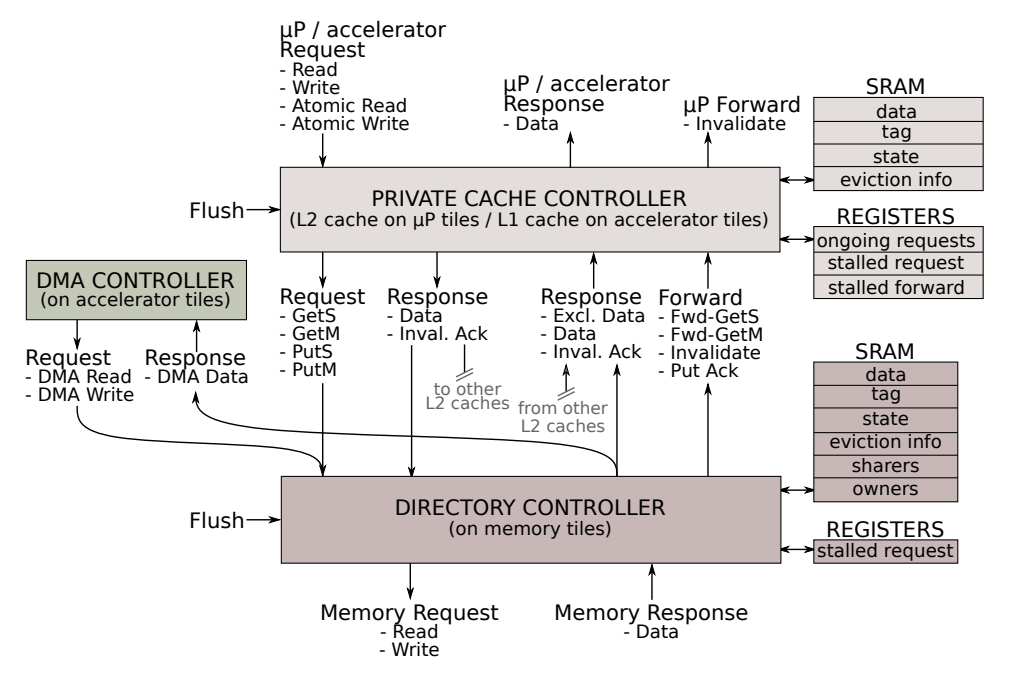
\includegraphics[width=1\columnwidth]{fig/esp_hier.png}
  \caption{ESP Cache Hierarchy~\cite{giri18}}
  \label{fig:esp_hier}
  \end{figure}

\begin{figure}[h]
  \centering
  \captionsetup{justification=centering, format=hang}
  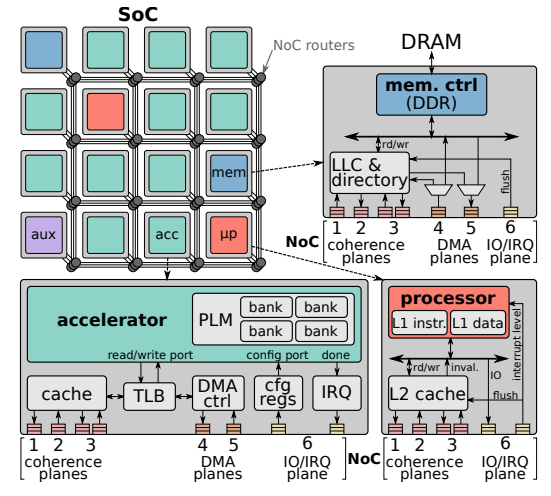
\includegraphics[width=1\columnwidth]{fig/noccache.png}
  \caption{Detailed ESP Tile Grid~\cite{giri18}}
  \label{fig:esp_tile}
  \end{figure}

